Nei capitoli precedenti sono stati introdotti i concetti teorici e operativi necessari alla realizzazione del progetto. In particolare nel Capitolo 1 sono stati descritti i fondamenti geometrici e matematici alla base della rappresentazione e manipolazione di oggetti 3D, mostrando come mesh, trasformazioni e sistemi di coordinate permettano di modellare e controllare il movimento nello spazio tridimensionale. Nel capitolo 2, invece, è stato analizzata la pipeline di animazione attraverso tool e software specifici, soffermandosi sul rigging, sullo skinning e sulle tecniche di acquisizione e trasferimento del movimento tramite sistemi di motion capture.

In questo capitolo tali conoscenze vengono applicate nella costruzione del workflow sviluppato per la presente tesi. L'obbiettivo è automatizzare il trasferimento di animazioni umanoidi verso modelli non convenzionati, riducendo l'intervento manuale e rendendo il processo più efficiente e scalabile. Verranno quindi illustrate le fasi operative che compongono la pipeline: a partire dell'importazione e test delle animazioni umanoidi, passando per la generazione automatica dello scheletro e l'assegnazione dei pesi alla mesh, fino al retargeting dell'animazione e all'integrazione finale in Unity. Ogni sezione descriverà sia gli strumenti utilizzati sia gli script utilizzati, mettendo in evidenza le scelte progettuali adottate e i risultati ottenuti.

\section{Importazione dei modelli umanoidi}

L'importazione del modello 3D rappresenta il primo passo fondamentale nel processo di animazione di un personaggio umanoide. Affinché un modello possa essere animato correttamente, esso deve essere dotato di una struttura scheletrica interna (rig) che consenta la manipolazione delle articolazioni e la deformazione della mesh. La qualità e la correttezza dei rig influenzano direttamente la fluidità e la naturalezza dei movimenti, rendendo questa fase cruciale per l'intera pipeline di animazione.

In ambito di sviluppo videoludico e applicazioni interattive, i modelli umanoidi vengono generalmente importati da librerie esterne o realizzati tramite software di modellazione 3D. Tuttavia, è necessario assicurarsi che il formato del file sia compatibile con il motore di sviluppo utilizzato: il formato FBX è il più diffuso in quanto permette di importare non solo la geometria del modello, ma anche la rig e, se presenti, le animazioni predefinite.

L'obiettivo di questa sezione è quindi descrivere i principali formati di file utilizzati, le fonti più comuni per l'acquisizione di modelli umanoidi e le impostazioni necessarie per garantire una corretta integrazione del personaggio all'interno dell'ambiente Unity.

\subsection{Tipologie di modelli (Mixamo, Unity Asset Store)}

Piattaforme come Mixamo e Unity Asset Store mettono a disposizioni personaggi già riggati, riducendo significativamente i tempi di preparazione e permettendo di concentrarsi sulla fase di animazione.

Mixamo, un servizio offerto da Adobe, mette a disposizione una libreria molto vasta di personaggi 3D completi di scheletro. La peculiarità di Mixamo risiede nel sistema di auto-rigging, che permette di applicare automaticamente uno scheletro umanoide a un modello caricato dall'utente.
L'Unity Asset Store, invece, è un marketplace integrato nel motore Unity, che offre modelli 3D sviluppati da artisti e studi professionisti. I modelli presenti nello store variano notevolmente in termini di complessità, qualità delle texture, dettaglio del rig e presenza o meno di animazioni incluse.

\begin{figure}[h]
\begin{center}
     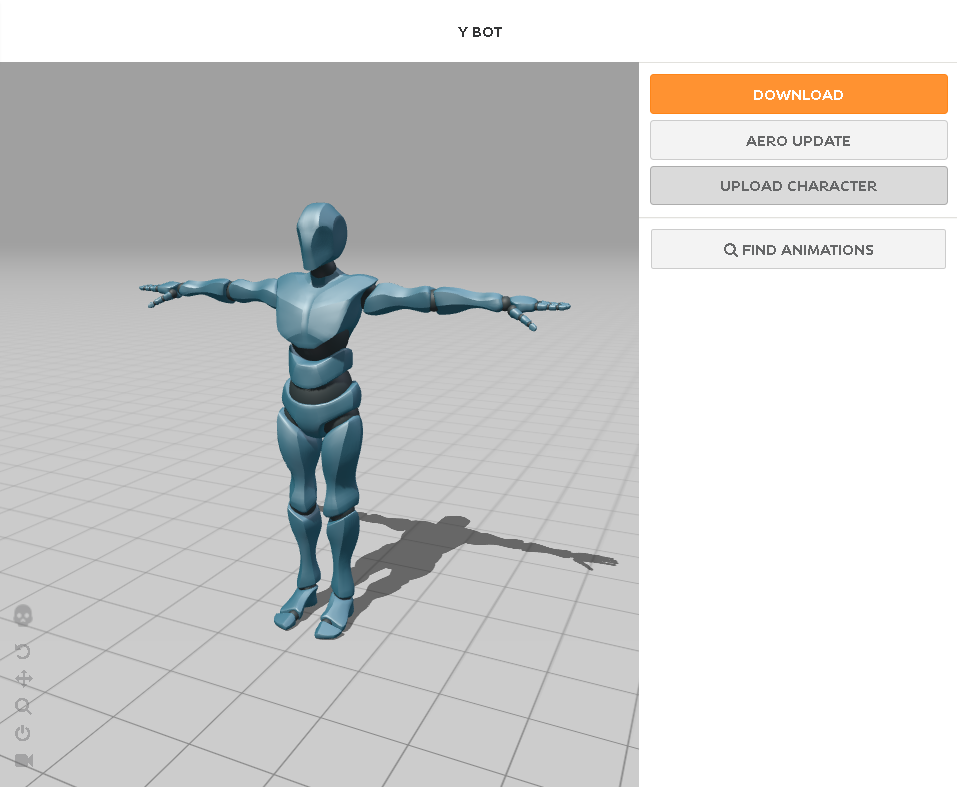
\includegraphics[width=10cm]{figure/mixamo2.png}
     \caption{Impostazione animazione su Mixamo}
\end{center}
\end{figure}

\subsection{Formati supportati (FBX, OBJ)}

Nella fase di importazione dei modelli umanoidi in Unity, il formato del file riveste un ruolo fondamentale, poiché determina quali informazioni saranno effettivamente trasferite all'interno del progetto. I due formati più utilizzati in questo contesto sono FBX  e OBJ, ciascuno caratterizzato da specifiche funzionalità e limiti.

Il formato FBX (Filmbox) è considerato lo standard nell'ambito dell'animazione 3D e della produzione videoludica. Oltre alla mesh del modello, l'FBX è in grado di contenere al suo interno la struttura scheletrica (rig), le animazioni associate, le informazioni sui materiali e le texture. Grazie a queste caratteristiche, l'FBX permette di trasferire un modello completo direttamente da software di modellazione come Blender, AutoCAD Maya (come in figura ~\ref{fig:auto}) o 3ds Max a Unity, mantenendo intatta la gerarchia delle ossa e la corretta disposizione delle animazioni.
Al contrario, il formato OBJ è molto più semplice e limitato. Esso rappresenta esclusivamente la geometria della mesh, senza contenere rig né animazioni. Questo lo rende adatto per modelli statici o come base per successivi processi di rigging e animazione, ma non per una importazione diretta di personaggi già animabili.

\begin{figure}[h]
\begin{center}
     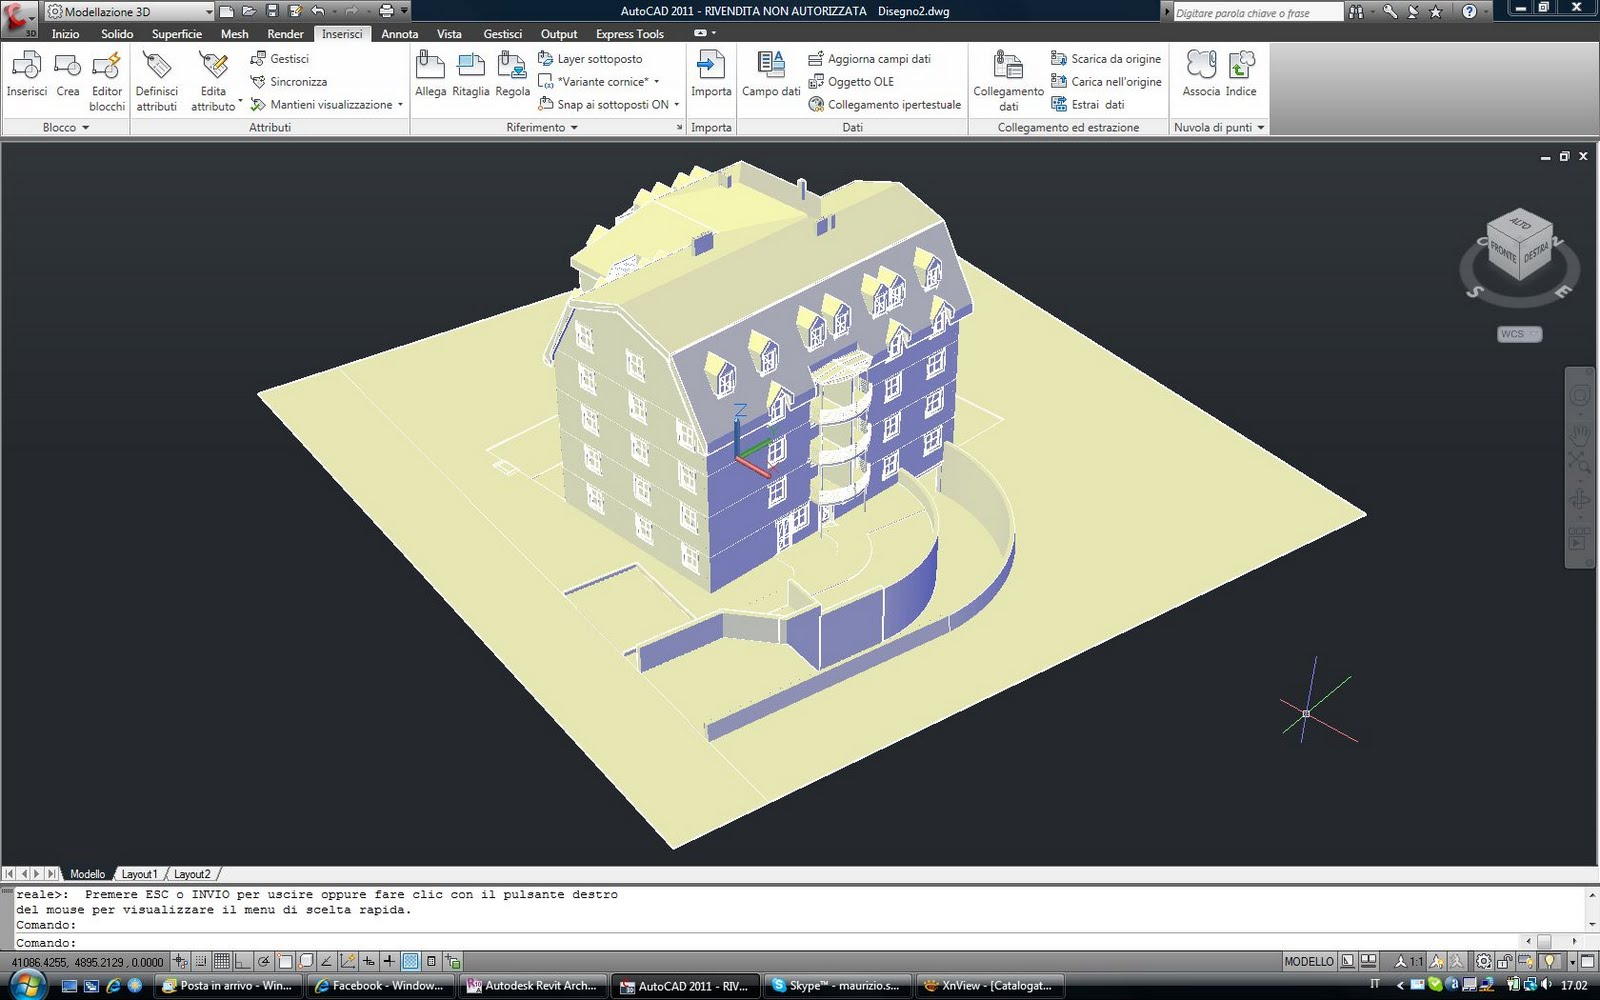
\includegraphics[width=12cm]{figure/autocad.png}
     \caption{Formato FBX utilizzato anche su AutoCAD}
     \label{fig:auto}
\end{center}
\end{figure}

In questa fase, l'obiettivo principale è garantire che il modello umanoide sia pronto per ricevere animazioni, senza intervenire ancora su rigging, skinning o retargeting automatico, che saranno approfonditi nei capitoli successivi.

\section{Applicazione di animazioni predefinite}

Una volta importato il modello umanoide nell'ambiente di sviluppo, è possibile procedere con l'applicazione delle animazioni. L'utilizzo di animazioni predefinite consente di ridurre notevolmente i tempi di produzione, evitando la necessità di creare manualmente i movimenti tramite tecniche di keyframing o sistemi di motion capture. Le animazioni predefinite sono generalmente organizzate in librerie, come quelle messe a disposizione da Mixamo, dall'Unity Asset Store o da altri archivi professionali di motion data.

Unity facilita l'integrazione delle animazioni attraverso il sistema di configurazione del rig Humanoid, che permette di adattare automaticamente le animazioni anche tra modelli differenti. Ciò significa che una stessa animazione, se correttamente configurata, può essere riutilizzata su più personaggi, a condizione che dispongano di una struttura scheletrica compatibile.

\subsection{Animazioni di base: camminata, corsa, salti}

Le animazione considerate "base" sono quelle che descrivono le azioni fondamentali del movimento umano. Tra le più comuni si trovano:

\begin{itemize}
    \item \textbf{Idle}: posizione di riposo del personaggio
    \item \textbf{Walk cycle}: ciclo completo di camminata.
    \item \textbf{Run cycle}: ciclo di corsa, caratterizzato da maggiore ampiezza e ritmo del movimento.
    \item \textbf{Jump}: animazione di salto, tipicamente suddivisa in tre fasi (preparazione, fase aerea e atterraggio).
\end{itemize}

\begin{figure}[H]
\centering
\begin{subfigure}{0.48\textwidth}
  \centering
  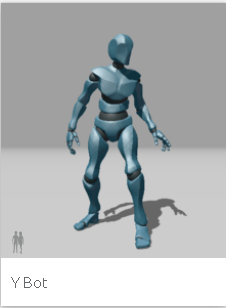
\includegraphics[height=4cm, keepaspectratio]{figure/Y-bot.png}
  \caption{Y-bot}
\end{subfigure}\hfill
\begin{subfigure}{0.48\textwidth}
  \centering
  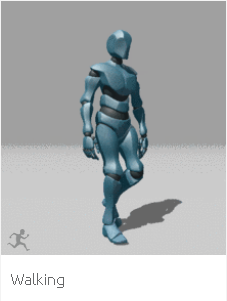
\includegraphics[height=4cm, keepaspectratio]{figure/walk.png}
  \caption{walking}
\end{subfigure}

\vspace{0.6em}

\begin{subfigure}{0.48\textwidth}
  \centering
  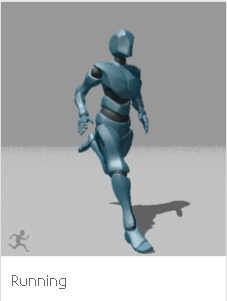
\includegraphics[height=4cm, keepaspectratio]{figure/run.png}
  \caption{Running}
\end{subfigure}\hfill
\begin{subfigure}{0.48\textwidth}
  \centering
  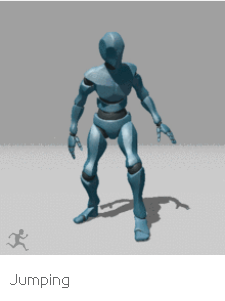
\includegraphics[height=4cm, keepaspectratio]{figure/jump.png}
  \caption{Jumping}
\end{subfigure}
\caption{Animazioni base.}
\end{figure}



Queste animazioni costituiscono la base per il controllo del personaggio in un ambiente interattivo, come un videogioco o una simulazione. Durante l'importazione delle clip, Unity consente di analizzare e modificare le proprietà delle animazioni, come la ripetizione ciclica (loop), la sincronizzazione dei piedi o la gestione del movimento della radice (root motion), migliorando la fluidità e la naturalezza del risultato finale.

\subsection{Librerie di animazioni e compatibilità con i rig}

Le librerie di animazioni predefinite possono variare per stile, complessità e struttura scheletrica di supporto. Quando si utilizza una libreria, è importante assicurarsi che l'animazione sia compatibile con il rig del modello. Unity supporta questa operazione tramite il sistema di retargeting Humanoid, che consente di adattare le animazioni a scheletri differenti mantenendo la corretta corrispondenza anatomica tra le ossa.

Se il modello e l'animazione sono entrambi configurati come Humanoid, Unity può applicare automaticamente l'animazione anche se proviene da un personaggio con proporzioni diverse. In caso contrario (ad esempio con rig personalizzati o non umani), è necessario intervenire manualmente sulla mappatura delle ossa o utilizzare strumenti esterni di rigging ed editing dell'animazione.

In questo modo, l'adozione della libreria di animazioni predefinite consente di ottenere risultati rapidi e coerenti, permettendo di concentrare gli sforzi creativi sulla logica di interazione e sul comportamento del personaggio piuttosto che sulle fasi dettagliate di creazione del movimento.

\section{Pipeline di integrazione animazione}

L'integrazione delle animazioni all'interno di Unity si basa su una pipeline strutturata che consente di importare correttamente il modello umanoide, configurarne il rig, associare le clip di animazione e gestirne la transizione durante l'esecuzione dell'applicazione. Tale processo assume un ruolo centrale nello sviluppo di personaggi interattivi, perché definisce il modo in cui le animazioni vengono interpretate e riprodotte dal motore grafico. La pipeline può essere suddivisa in diverse fasi consecutive (come rappresentato in figura ~\ref{fig:pipe}), che vanno dall'esportazione del modello da un software esterno fino alla definizione della logica di controllo dei movimenti attraverso l'\textbf{Animator Controller}.

\begin{figure}[H]
\begin{center}
     \centering
     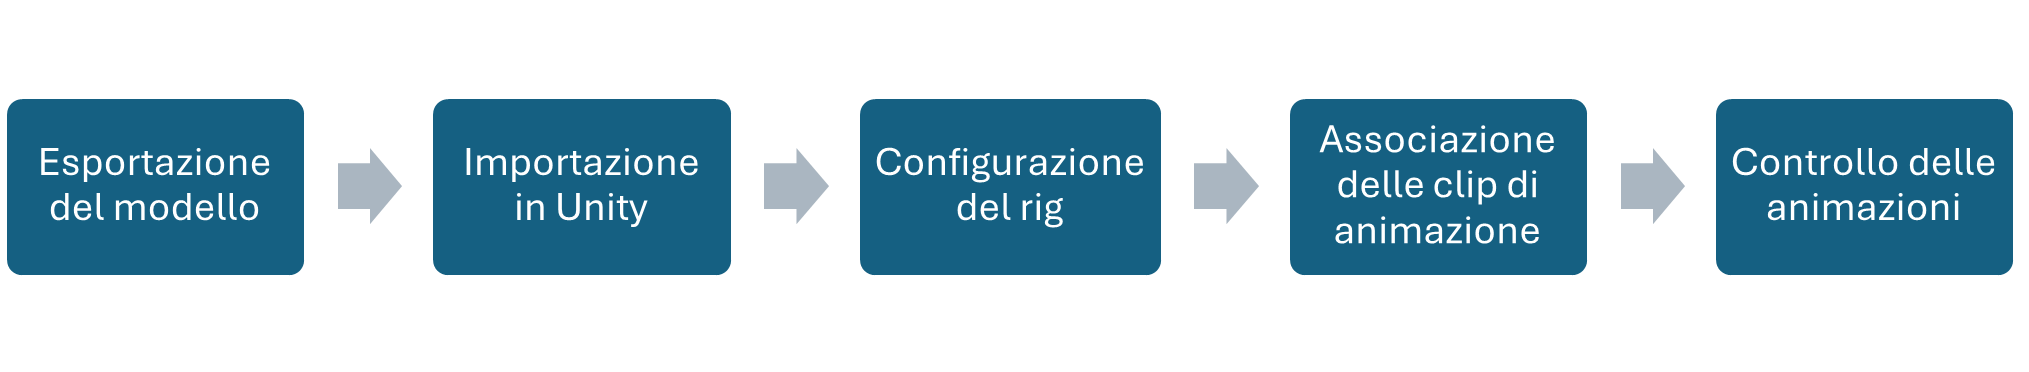
\includegraphics[width=0.85\linewidth]{figure/pipe.png}
     \caption{Pipeline di integrazione animazione}
     \label{fig:pipe}
\end{center}
\end{figure}

\subsection{Esportazione e importazione del modello (FBX $\rightarrow$ Unity)}

Il primo passaggio consiste nell'esportazione del modello e delle relative animazioni da un software di modellazione 3D o da un piattaforma di librerie come Mixamo. Il formato maggiormente utilizzato è FBX, in quanto consente di preservare la struttura gerarchica dello scheletro, le pesature dei vertici e le curve di animazione associate.

Una volta inserito il file FBX all'interno del progetto Unity, il motore provvede alla sua conversione automatica nel formato interno. A questo punto, l'utente può accedere al pannello delle \textbf{Import Settings} (Figura~\ref{fig:confi}), che consente di definire la tipologia di rig tramite l'impostazione \textbf{Humanoid}, garantendo così la compatibilità con il sistema di retargeting del motore. Inoltre, nella sezione Animation, è possibile separare le clip contenute nel file, attivarne il loop, normalizzarne la durata o abilitare l'opzione \textbf{Root Motion} (Figura~\ref{fig:inspe}), che influenzerà la gestione del movimento nello spazio tridimensionale.

\begin{figure}[h]
\begin{center}
     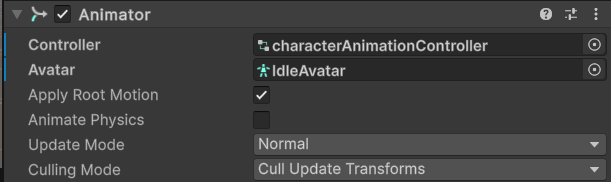
\includegraphics[width=12cm]{figure/inspe.png}
     \caption{Proprietà di un oggetto selezionato}
     \label{fig:inspe}
\end{center}
\end{figure}

\textbf{Proprietà dell'oggetto selezionato}
\begin{enumerate}
    \item \textbf{Controller}: il Animation Controller collegato all'oggetto.
    \item \textbf{Avatar}: l'Avatar per questo personaggio (se l'Animatore viene usato per animare un personaggio umanoide).
    \item \textbf{Apply Root Motion}: seleziona se controllare la posizione e la rotazione del personaggio dall'animazione stessa o dallo script.
    \item \textbf{Update Mode}: questo ti permette di selezionare quando l'Animator aggiorna e quale scala temporale deve utilizzare
    \begin{enumerate}
        \item \textbf{Normale}: L'Animator viene aggiornato in sincronia con la chiamata Update, e la velocità dell'animatore corrisponde a quella attuale. Se la scala temporale è rallentata, le animazioni rallenteranno per adattarsi.
        \item \textbf{Animate Physics}: L'animatore viene aggiornato in sincronia con la chiamata FixedUpdate (cioè in perfetta sincronia con il sistema fisico). Dovresti usare questa modalità se stai animando il movimento di oggetti con interazioni fisiche, come i personaggi che possono spingere oggetti rigidbody.
        \item \textbf{Unscaled Time}: L'animatore viene aggiornato in sincronia con la chiamata Update, ma la velocità dell'animatore ignora la scala temporale attuale e anima comunque al 100\% della velocità. Questo è utile per animare un sistema GUI a velocità normale usando scale temporali modificate per effetti speciali o per mettere in pausa il gameplay.
    \end{enumerate}
    \item \textbf{Culling Mode}: la modalità culling puoi scegliere per le animazioni.
    \begin{enumerate}
        \item \textbf{Always animate}: animare sempre, non fare culling anche fuori campo.
        \item \textbf{Cull Update Transforms}: Retarget, IK e scrittura delle trasformazioni sono disabilitate quando i renderer non sono visibili.
        \item \textbf{Cull Completely}: l'animazione è completamente disabilitata quando i renderer non sono visibili.
    \end{enumerate}
    
\end{enumerate}

\subsection{Animator Controller e gestione degli stati di animazione}

Una volta importate le animazioni, è necessario definire le modalità con cui il personaggio passerà da un movimento all'altro durante l'esecuzione. Unity utilizza a tal fine l'\textbf{Animator Controller} (Figura ~\ref{fig:cont}), una macchina a stati finiti che rappresenta le diverse animazioni come nodi collegati da transizioni. Ogni transizione può essere controllata tramite parametri (booleani, interi, float o trigger), modificabili a runtime tramite script o input dell'utente.

Questo approccio consente di gestire in modo modulare e scalabile sequenze complesse di movimenti, come la transizione fluida tra camminata e corsa o la sincronizzazione tra salto e atterraggio. Inoltre, Unity mette a disposizione strumenti avanzati come i \textbf{Blend Trees}, che permettono di interpolare più animazioni in funzione di un parametro continuo (ad esempio la velocità), garantendo una maggiore naturalezza nell'esecuzione delle animazioni di locomozione.

Un'architettura dell'Animator Controller ben progettata consente quindi una maggiore flessibilità, favorisce il riutilizzo delle animazioni e semplifica l'eventuale estensione futura del sistema di controllo del personaggio.

\begin{figure}[H]
\begin{center}
     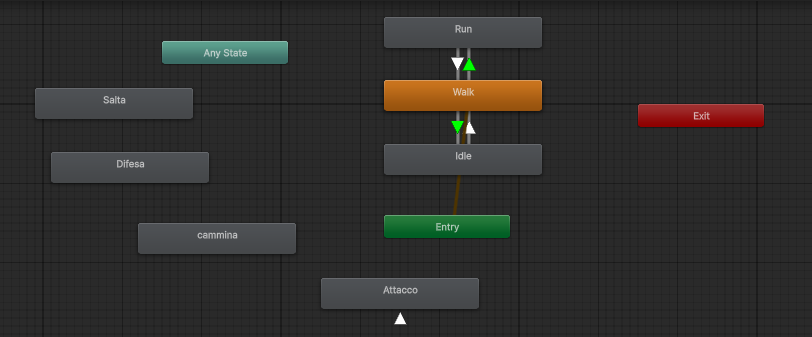
\includegraphics[width=12cm]{figure/controller.png}
     \caption{Animation Controller con diverse animazioni}
     \label{fig:cont}
\end{center}
\end{figure}

\section{Gestione dei modelli animati}

Nel progetto sviluppato, la gestione del modello umanoide risulta semplificata dal fatto che il personaggio utilizzato era già dotato di rig completo e di corretta associazione tra mesh e scheletro. Pertanto, non è stato necessario intervenire sul processo di \textit{skinning} o sulla definizione dei pesi dei vertici, operazioni che normalmente richiederebbero l'utilizzo del software di rigging come Blender o Maya. Unity ha riconosciuto automaticamente la struttura scheletrica del modello e ha provveduto  a configurarla secondo il sistema \textbf{Humanoid}, permettendo così di applicare animazioni predefinite senza ulteriore modifiche.

La riproduzione delle animazioni è stata gestita tramite l'\textbf{Animator Controller}, che ha permesso di definire e controllare le transizioni tra i diversi stati animati, come ad esempio il passaggio da idle a camminata o corsa. Poiché il modello era già predisposto per l'utilizzo delle animazioni umane standard, l'applicazione delle clip è avvenuta in modo diretto, senza la necessità di operazioni di retargeting manuale o adattamento delle pose.

Queste condizione ha semplificato la pipeline di animazione, rendendo il processo più rapido ed efficiente. Rispetto a modelli non organici o non riggati, dove sarebbe necessario costruire uno scheletro artificiale e definire le influenze delle ossa sulla superficie della mesh, nel caso degli umanoidi la struttura preesistente consente un'applicazione immediate e riutilizzabile delle animazioni.

In sintesi, l'utilizzo di un modello già riggato e compatibile con il sistema Humanoid di Unity ha permesso di concentrarsi esclusivamente sulla gestione dell'Animator Controller e delle animazioni, semplificando notevolmente il flusso di lavoro rispetto a oggetti non animati o con rig personalizzato.


\section{Retargeting su umanoidi}

Il retargeting è una procedura che consente di applicare la stessa animazione a modelli diversi, purché condividano una struttura scheletrica compatibile. Nel caso dei personaggi umanoidi, Unity dispone di un sistema di retargeting integrato basato sullo standard \textbf{Humanoid Rig}, che permette di trasferire animazioni tra modelli differenti mantenendo la coerenza dei movimenti. Questo processo risulta particolarmente utile quando si utilizzano librerie di animazioni esterne, come quelle fornite da Mixamo, oppure quando si integrano personaggi provenienti da diverse fonti di modellazione 3D (tipo MoveAI).  

\subsection{Concetto di retargeting tra rig simili}

Il sistema Humanoid di Unity definisce una mappatura standard delle principali articolazioni del corpo (test, colonna vertebrale, braccia, gambe, mani). Quando il modello viene importato e configurato come Humanoid, Unity riconosce automaticamente l'equivalente dello scheletro intero e consente di utilizzare animazioni create per altri personaggi umanoidi.
In termini pratici, ciò significa che un'animazione di camminata può essere applicata a qualsiasi modello umanoide senza la necessità di ricreare manualmente il movimento.

\subsection{Metodi automatici semplificati (solo per personaggi umanoidi)}

Unity gestisce il retargeting in modo quasi completamente automatico. È sufficiente:

\begin{enumerate}
    \item Importare il modello come \textbf{Humanoid Rig}
    \item Associare una clip di animazione proveniente da un'altra sorgente
    \item Applicarla tramite l'\textbf{Animator Controller}
\end{enumerate}

Grazie a questa funzione, è possibile riutilizzare un'ampia gamma di animazioni già presenti nelle librerie, riducendo significativamente il tempo richiesto per la produzione di movimenti realistici.

\begin{figure}[H]
\begin{center}
     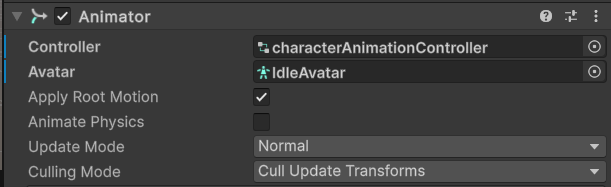
\includegraphics[width=12cm]{figure/retar.png}
     \caption{Applicazione animazioni create per un modello}
     \label{fig:retar}
\end{center}
\end{figure}

\subsection{Limitazioni rispetto a oggetti non organici}

Il retargeting automatico presente nei software moderni (es. Blender, Unity, MotionBlender) si basa quasi sempre su un modello \textbf{umanoide standardizzato}, caratterizzato da un struttura scheletrica prevedibile (colonna vertebrale, braccia, gambe, testa) e da vincoli cinematici tipici dell'anatomia umana.

Quando l'oggetto da animare \textbf{non possiede caratteristiche antropomorfe}, questa pipeline non risulta applicabile o perde grande parte della sua efficacia. Oltre ai casi già citati (creature non umanoidi, oggetti meccanici, strutture articolate atipiche), esistono varie categorie problematiche:

Perché il retargeting automatico fallisce:
\begin{enumerate}
    \item \textbf{Assenza di una corrispondenza diretta tra giunti}.
    I sistemi umanoide prevedono un mapping "uno-a-uno" tra ossa equivalenti (Hips $\rightarrow$ Hips, Spine $\rightarrow$ Spine, ecc.).
    
    \item \textbf{Topologia scheletrica non compatibile}.
    Creature multipedali, insetti, robot od oggetti inventati presentano:
    \begin{itemize}
        \item più arti o meno arti
        \item articolazioni non lineari (segmenti meccanici, giunti cilindrici, pistoni, tentacoli)
        \item strutture non gerarchiche
    \end{itemize}
    \item \textbf{Range di movimento non umano}.
    Gli algoritmi umanoidi assumono vincoli cinematici:
    \begin{itemize}
        \item cavallo pelvico
        \item limitazioni di abduzione/adduzione
        \item articolazioni sferiche/hinge
            Oggetti artificiali possono violare tutti questi limiti (rotazione 360 gradi, assi multipli, traslazioni)
    \end{itemize}
    \item \textbf{Root motion non universale}.
    Il movimento radice negli umanoidi è centrato su Hips/Pelvis. In un robot o in una creatura aliena, la "root" può essere ovunque.
\end{enumerate}

\section{Gestione dei modelli inanimati}

Nel caso degli oggetti inanimati, la gestione dell'animazione ha richiesto un flusso di lavoro più articolato rispetto a quello adottato per il modello umanoide, in quanto i modelli utilizzati non erano originariamente dotati di uno scheletro nè di un sistema di skinning. Di conseguenza, è stato necessario procedere con l'implementazione automatica del rigging e dello skinning, al fine di rendere gli oggetti animabili all'interno dell'ambiente di sviluppo.

Il processo ha previsto la generazione di una struttura scheletrica artificiale, composta da un insieme di ossa funzionali al tipo di movimento desiderato. Successivamente, è stata applicata una procedura di skinning automatico, che ha permesso di associare la mesh alle ossa generate, distribuendo i pesi dei vertici in modo coerente senza interventi manuali. Questa fase, sebbene automatizzata , risulta fondamentale per garantire una deformazione corretta dell'oggetto durante l'animazione.

\section{Preparazione dei modelli}

La preparazione dei modelli costituisce un passaggio fondamentale nella pipeline di animazione 3D, poiché determina sia la struttura geometrica degli oggetti sia la configurazione dello scheletro necessario per il loro movimento. In questo capitolo, si descrive il processo seguito per la creazione di modelli modulari e per la generazione automatica di un rigging iniziale utilizzando \textbf{Blender} come ambiente di lavoro principale.

L'obiettivo di questa fase è duplice: da un lato, garantire che le mesh siano organizzate e pronte per essere animate; dall'altro, creare uno scheletro coerente e funzionale, in grado di supportare deformazioni realistiche e di integrarsi con animazioni predefinite. Per facilitare questo processo, sono stati impiegati riferimenti a scheletri umanoidi standard, adattati alle specificità dei modelli utilizzati.

\subsection{Descrizione della mesh}

La fase di definizione delle mesh costituisce il primo passo nella preparazione dei modelli per l'animazione in Blender. In questo lavoro, i modelli sono stati realizzati in forma modulare, al fine di consentire una gestione semplice e flessibile delle diverse componenti durante la fase di rigging, skinning e animazione.

I modelli principali utilizzati sono i seguenti: 
\begin{itemize}
    \item \textbf{Piatto con gambe}: rappresenta una struttura base costituita da una mesh piana (piatto) che funge da corpo principale, integrata con due gambe posizionate simmetricamente per consentire il movimento verticale e traslatorio. Questa configurazione permette di testare deformazioni e animazioni di base come camminata o rotazioni.
    \item \textbf{Piattino con tazzina e gambe}: questa combinazione rappresenta una forma più complessa, in cui la tazzina è posizionata sopra il piattino, entrambi supportati da due gambe. Tale struttura offre un maggiore livello di articolazione e permette di sperimentare il comportamento delle mesh durante animazioni più complesse, simulando un personaggio modulare con elementi sovrapposti.
\end{itemize}

Ogni mesh è stata importata in Blender come oggetto separato, con una propria origine e pivot point, per facilitare l'allineamento con lo scheletro e garantire una corretta deformazione durante l'animazione. L'approccio modulare consente inoltre di sostituire o modificare singoli componenti senza compromettere l'intera struttura del modello.

\begin{figure}[h]
\centering
\begin{subfigure}{0.45\textwidth}
    \centering
    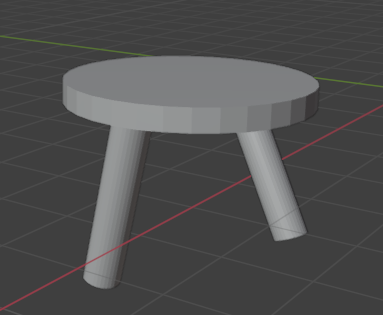
\includegraphics[width=\linewidth]{figure/piatto.png}
    \caption{Piatto con gambe}
\end{subfigure}
\hfill
\begin{subfigure}{0.45\textwidth}
    \centering
    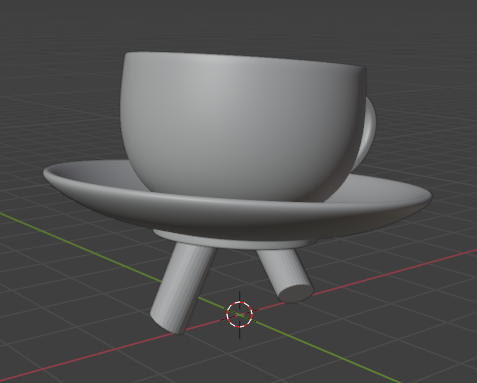
\includegraphics[width=\linewidth]{figure/tazza.png}
    \caption{Piattino con tazzina e gambe}
\end{subfigure}
\caption{Mesh dei modelli in Blender}
\end{figure}

\subsection{Creazione dello scheletro iniziale (da rig umanoide)}

La definizione dello scheletro iniziale rappresenta il passaggio fondamentale per consentire l'animazione di un modello. Lo \textbf{scheletro}, o \textit{rig}, è costituito da una struttura gerarchica (Figura ~\ref{fig:gera}) di ossa che permette la deformazione controllata delle mesh durante il movimento. La scelta di utilizzare un \textbf{rig umanoide come riferimento}, come si evidenza in figura ~\ref{fig:scheletro}, deriva dalla necessità di disporre di una struttura articolare coerente, facilmente adattabile a modelli anche non antropomorfi.

Un rig umanoide standard generalmente composto da elementi ricorrenti, quali:
\begin{itemize}
    \item una colonna strutturale centrale (spina dorsale);
    \item due arti inferiori con articolazione dell'anca, del ginocchio e della caviglia;
    \item due arti superiori con articolazione della spalla, del gomito e del polso;
    \item un nodo centrale di orientamento (pelvis o root).
\end{itemize}

\begin{figure}[H]
\begin{center}
     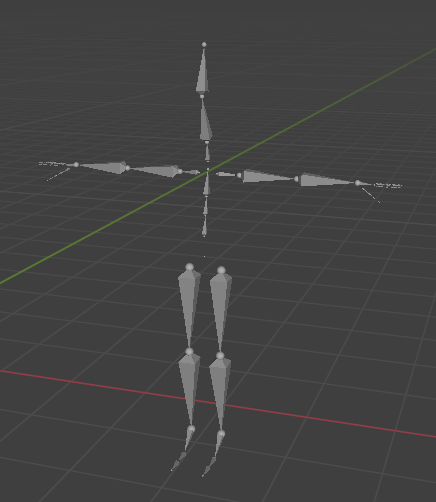
\includegraphics[width=7cm]{figure/scheletro.png}
     \caption{Struttura gerarchica} \label{fig:scheletro}
\end{center}
\end{figure}

Sebbene i modelli trattati in questo lavoro non riproducano figure umane, la \textbf{logica articolare umanoide} risulta comunque utile. Le "gambe" dei modelli, infatti, devono essere in grado di simulare movimenti come passo, flessione o rotazione, che trovano un riferimento diretto nelle articolazioni del corpo umano.

\begin{figure}[H]
\begin{center}
     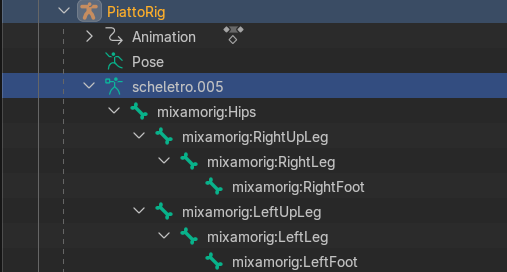
\includegraphics[width=10cm]{figure/gerar.png}
     \caption{Struttura scheletrica che viene presentato quando se importa uno scheletro su Blender} \label{fig:gera}
\end{center}
\end{figure}

L'adozione di una \textbf{struttura scheletrica standardizzata} offre inoltre due vantaggi rilevanti:
\begin{enumerate}

    \item \textbf{Compatibilità con librerie di animazioni esistenti:}

    Un rig umanoide consente di utilizzare animazioni già pronte, riducendo la necessità di creare ogni movimento manualmente.
    \item \textbf{Facilità di adattamento (retargeting):}

    la corrispondenza tra ossa standard rende possibile trasferire animazioni da un modello all'altro, anche quando le proporzioni o le forme sono differenti.
\end{enumerate}

In sintesi, la creazione dello scheletro iniziale si basa sulla definizione di una struttura ossea coerente, gerarchica e compatibile con sistemi di animazione già esistenti. Nel punto successivo verrà descritta l'applicazione pratica di questo processo.

\section{Implementazione del rigging automatico in Blender}

La generazione automatica di scheletri tridimensionali rappresenta una delle problematiche centrali nell'ambito dell'animazione digitale. Essa consiste nel definire una struttura articolata che consenta di deformare in modo realistico una mesh 3D durante il movimento. La predizione di una struttura scheletrica valida a partire da una mesh tridimensionale è un compito complesso, in quanto richiede di catturare sia la geometria sia la topologia dell'oggetto, mantenendo relazioni coerenti tra le diverse articolazioni.

I metodi tradizionali di rigging automatico si basano spesso su modelli o schemi predefiniti, progettati per una gamma limitata di morfologie. Tuttavia, tali approcci risultano poco flessibili e mostrano difficoltà nel gestire modelli con strutture non convenzionali o topologie molto diverse da quelle umane. Per superare questi limiti, le ricerche più recenti hanno proposto approcci di tipo \textbf{sequenziale} o \textbf{autoregressivo}, in cui lo scheletro viene generato passo dopo passo, prevedendo la posizione di ogni nuovo giunto in relazione a quelli già creati. In questo modo, la costruzione della struttura ossea tiene conto della dipendenza gerarchica tra le articolazioni e della forma complessiva della mesh, garantendo una maggiore coerenza del risultato finale.

Un ulteriore problema affrontato da tali metodi riguarda la rappresentazione computazionale dello scheletro. Rappresentare una struttura gerarchica in un formato sequenziale non è banale, poiché occorre descrivere sia le coordinate spaziali delle ossa sia le relazioni di parentela tra esse. Soluzioni semplicistiche, che ordinano le ossa secondo percorsi predefiniti, possono introdurre ridondanza e inefficienze, oltre a rendere difficile il rispetto dei vincoli strutturali.

Per gestire in modo efficace queste relazioni, alcuni approcci moderni propongono tecniche di \textbf{codifica strutturale} che discretizzano le informazioni spaziali e gerarchiche dello scheletro, in modo da preservarne la coerenza tipologica. Tali strategie consentono di ottenere scheletri più flessibili, adattabili e correttamente articolati, anche nel caso di modelli non organici o con forme atipiche.

I principi teorici alla base di queste metodologie hanno fornito la base concettuale per lo sviluppo di procedure automatizzate di rigging, come quelle realizzata in Blender mediante script Python, descritta nella sezione successiva.


\subsection{Generazione dello scheletro adattato all'oggetto}

A partire dai principi teorici descritti nella sezione precedente, è stata sviluppata una procedura di \textbf{rigging automatico} all'interno di \textit{Blender}, con l'obiettivo di generare in modo semi-automatizzato lo scheletro di oggetti tridimensionali non convenzionali, come un piatto o una tazzina dotati di gambe. Il processo è stato realizzato attraverso uno script \textit{Python} personalizzato, concepito per adattare un rig umanoide esistente alla morfologia del nuovo modello, riducendo l'intervento manuale richiesto nel rigging tradizionale.

Il metodo di implementazione prevede diverse fasi operative:

\begin{figure}[H]
\begin{center}
     \centering
     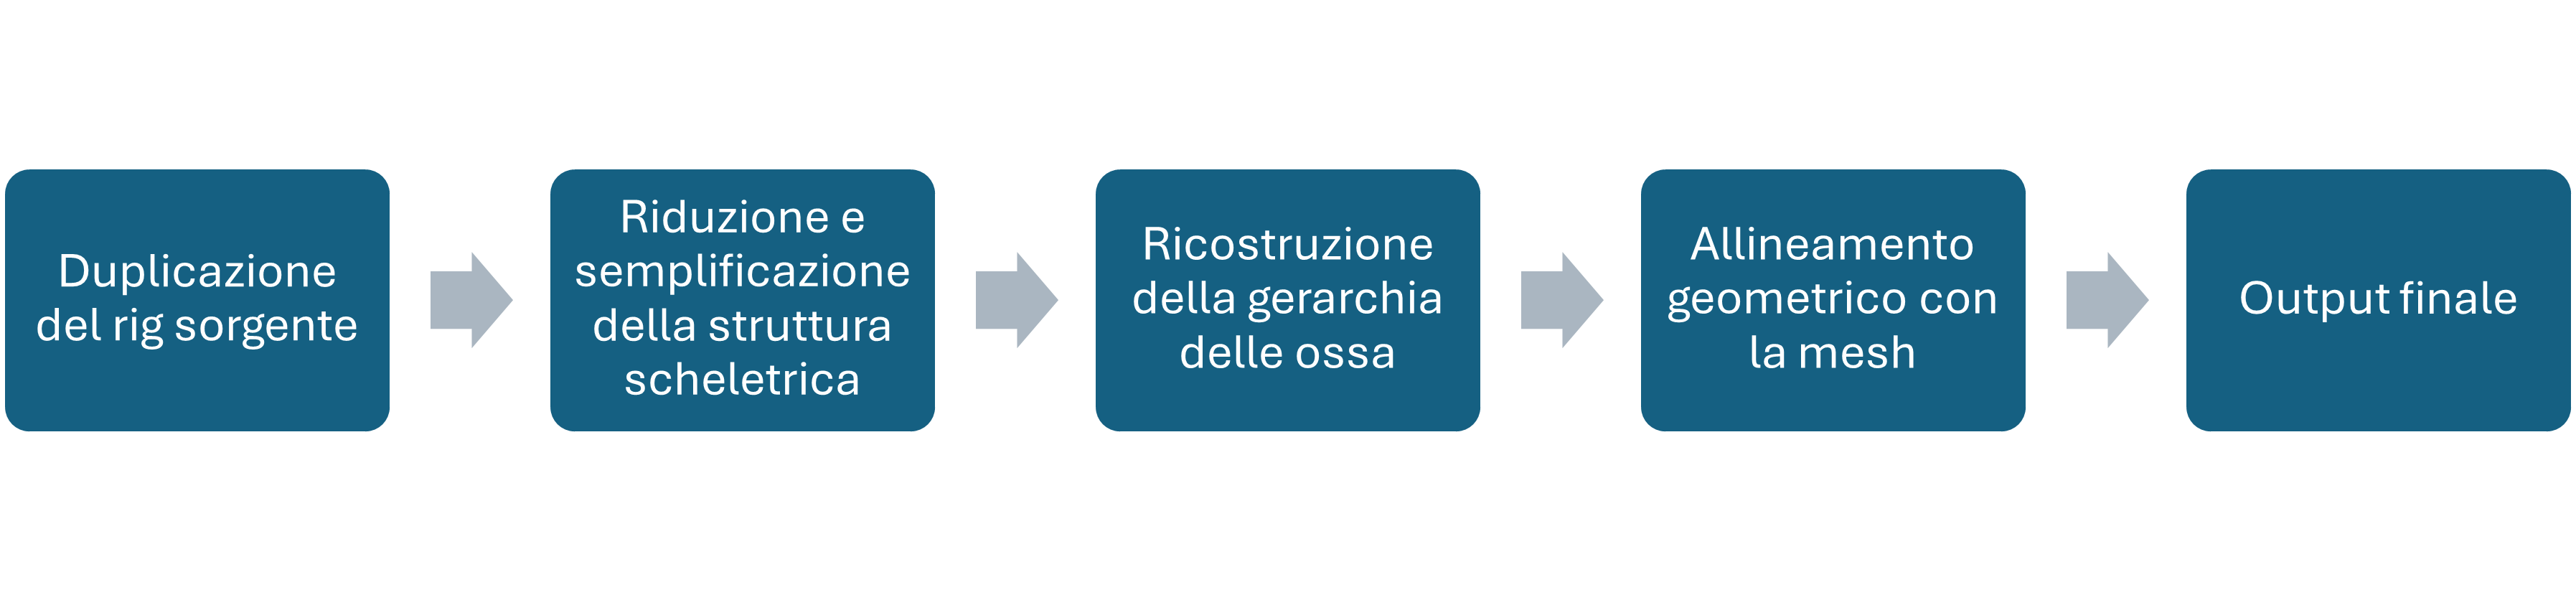
\includegraphics[width=0.85\linewidth]{figure/fasi.png}
     \caption{Fasi per la generazione dello scheletro}
     \label{fig:pipe}
\end{center}
\end{figure}
Queste fase operative presentate saranno spiegate successivamente.

\begin{enumerate}
    \item \textbf{Duplicazione del rig sorgente}

    Il punto di partenza è costituito da un rig umanoide di riferimento, già presente nella scena di Blender. Lo script ne crea una copia indipendente, mantenendone la struttura di base e i vincoli di orientamento. Questa operazione consente di preservare l'integrità del modello sorgente e di riutilizzare la sua gerarchia ossea come struttura iniziale per il nuovo oggetto.

    \vspace{5mm}
    \begin{minipage}{1\linewidth}
    \small
    \begin{algorithm}[H]
    \caption{DuplicateSourceRig}
    \label{alg:duplicate_rig}
    
    \KwIn{sourceRig, newRigName}
    
    \tcp{sourceRig: nome dell’armatura sorgente}
    \tcp{newRigName: nome della nuova armatura}
    
    src $\leftarrow$ getObjectFromScene(sourceRig)\;
    \tcp{Recupera l’oggetto armatura sorgente dalla scena}
    
    \If{src does not exist}{
        raise Error("Rig sorgente non trovato")\;
        \tcp{Interrompe l’esecuzione se l’armatura non è presente}
    }
    
    plateRig $\leftarrow$ copyObject(src)\;
    \tcp{Crea una copia dell’oggetto armatura}
    
    plateRig.data $\leftarrow$ copyRigData(src.data)\;
    \tcp{Duplica i dati dell’armatura per evitare riferimenti condivisi}
    
    plateRig.name $\leftarrow$ newRigName\;
    \tcp{Assegna il nuovo nome all’armatura duplicata}
    
    linkObjectToScene(plateRig)\;
    \tcp{Collega la nuova armatura alla collezione attiva della scena}
    
    setActiveObject(plateRig)\;
    \tcp{Imposta la nuova armatura come oggetto attivo}
    
    \end{algorithm}
    \end{minipage}

    
    \item \textbf{Riduzione e semplificazione della struttura scheletrica}

    Poiché l'obiettivo è quello di animare un oggetto con caratteristiche morfologiche ridotte rispetto a un corpo umano, lo script elimina automaticamente le ossa non necessarie (braccia, colonna vertebrale, mani, ecc.), mantenendo soltanto la parte inferiore dei rig - anca, gamba e piedi - sufficiente per conferire al modello la possibilità di movimento e stabilità.
    \vspace{5mm} %5mm vertical space

    \vspace{5mm}
    \begin{minipage}{1\linewidth}
    \begin{algorithm}[H]
    \caption{KeepLowerBodyBones}
    \label{alg:keep_lower_body}
    
    \KwIn{plateRig}
    
    \tcp{Imposta l’armatura in modalità di modifica}
    SetMode(plateRig, EDIT)\;
    
    \tcp{Recupera l’insieme delle ossa in modalità edit}
    editBones $\leftarrow$ plateRig.getEditBones()\;
    
    \tcp{Definisce l’elenco delle ossa da mantenere}
    keepBones $\leftarrow \emptyset$\;
    
    addBone(keepBones, Hips)\;
    addBone(keepBones, LeftUpLeg)\;
    addBone(keepBones, LeftLeg)\;
    addBone(keepBones, LeftFoot)\;
    addBone(keepBones, RightUpLeg)\;
    addBone(keepBones, RightLeg)\;
    addBone(keepBones, RightFoot)\;
    
    \end{algorithm}
    \end{minipage}


    \vspace{5mm} %5mm vertical space
    \item \textbf{Ricostruzione della gerarchia delle ossa}

    Dopo la rimozione delle parti superflue, vengono ristabilite le connessioni parent-child tra le ossa rimanenti, preservando la sequenza logica "Hips $\rightarrow$ UpLeg $\rightarrow$ Leg $\rightarrow$ Foot". In questo modo il rig conserva una struttura coerente con il sistema di animazione di Blender e risulta pienamente compatibile con il motore di animazione.

    \vspace{5mm}
    \begin{minipage}{1\linewidth}
    \begin{algorithm}[H]
    \caption{RebuildBoneHierarchy}
    \label{alg:rebuild_hierarchy}
    
    \KwIn{editBones}
    
    \tcp{Ricostruisce le relazioni parent--child}
    \tcp{per garantire una corretta propagazione}
    \tcp{delle trasformazioni}
    
    \ForEach{side $\in$ \{Left, Right\}}{
    
        upLeg $\leftarrow$ editBones.get(side + "UpLeg")\;
        \tcp{Recupera l'osso della coscia}
    
        leg $\leftarrow$ editBones.get(side + "Leg")\;
        \tcp{Recupera l'osso della gamba}
    
        foot $\leftarrow$ editBones.get(side + "Foot")\;
        \tcp{Recupera l'osso del piede}
    
        hips $\leftarrow$ editBones.get("Hips")\;
        \tcp{Recupera l'osso dei fianchi}
    
        \If{upLeg exists \textbf{and} hips exists}{
            setParent(upLeg, hips)\;
            \tcp{Collega la coscia ai fianchi}
        }
    
        \If{leg exists \textbf{and} upLeg exists}{
            setParent(leg, upLeg)\;
            \tcp{Collega la gamba alla coscia}
        }
    
        \If{foot exists \textbf{and} leg exists}{
            setParent(foot, leg)\;
            \tcp{Collega il piede alla gamba}
        }
    }
    
    \end{algorithm}
    \end{minipage}
    
    \item \textbf{Allineamento geometrico con la mesh}

    Una volta semplificato e ricostruito, lo scheletro viene riposizionato in modo automatico in relazione alla mesh dell'oggetto. Lo script calcola il \textit{bounding box} della geometria e ne individua il centro, in modo da posizionare correttamente le articolazioni principali (anca e gambe) in base alla scala e alla simmetria dell'oggetto. Questa operazione consente di ottenere un rig proporzionato o perfettamente adattato al modello 3D.
    
    \vspace{5mm}
    \begin{minipage}{1\linewidth}
    \begin{algorithm}[H]
    \caption{AlignRigToPlateCenter}
    \label{alg:align_rig}
    
    \KwIn{plate, editBones}
    
    \tcp{Calcola i vertici del bounding box del piatto}
    bbox $\leftarrow$ GetBoundingBoxVertices(plate)\;
    
    \tcp{Calcola il centro del bounding box}
    center $\leftarrow$ ComputeCenter(bbox)\;
    
    \tcp{Calcola i limiti verticali del bounding box}
    minZ $\leftarrow$ GetMinZ(bbox)\;
    maxZ $\leftarrow$ GetMaxZ(bbox)\;
    
    \tcp{Calcola i limiti laterali del bounding box}
    minX $\leftarrow$ GetMinX(bbox)\;
    maxX $\leftarrow$ GetMaxX(bbox)\;
    
    \tcp{Recupera l'osso dei fianchi}
    hips $\leftarrow$ editBones.get(Hips)\;
    
    \tcp{Riposiziona testa e coda dell'osso dei fianchi}
    SetHead(hips, center)\;
    SetTail(hips, center + (0, 0, (maxZ - minZ) $\times$ 0.2))\;
    
    \tcp{Riposiziona le ossa delle cosce}
    \ForEach{(side, xOffset) $\in$ \{(Left, minX $\times$ 0.7), (Right, maxX $\times$ 0.7)\}}{
    
        upLeg $\leftarrow$ editBones.get(side + "UpLeg")\;
        \If{upLeg exists}{
            SetHead(upLeg, center + (xOffset, 0, 0))\;
        }
    }
    
    \end{algorithm}
    \end{minipage}

    \item \textbf{Output finale}

    Al termine dell'esecuzione dello script Python, viene generato uno \textbf{scheletro adattato alla geometria dell'oggetto}, con una gerarchia coerente e correttamente allineata alla mesh. In questa fase, tuttavia, il rig non è ancora completamente pronto per l'animazione, poiché \textbf{non è stato eseguito lo skinning}, ovvero il processo di associazione dei vertici della mesh alle ossa con pesi di influenza.
\end{enumerate}

\begin{figure}[H]
\begin{center}
     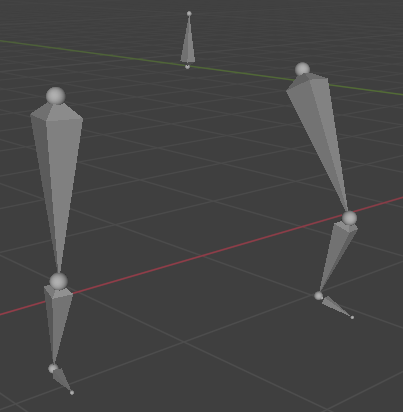
\includegraphics[width=6cm]{figure/piattoRig.png}
     \caption{Rig Umanoide} \label{fig:scheletro}
\end{center}
\end{figure}

L'approccio adottato rappresenta una versione semplificata dei metodi di rigging automatico più avanzati, traducendo in una procedura pratica alcuni dei principi teorici descritti nel capitolo precedente. Pur non implementando algoritmi di previsioni basati su modelli neurali o processi autoregressivi, lo script sviluppato in Blender consente di ottenere una \textbf{configurazione scheletrica adattativa}, riducendo in modo significativo i tempi di preparazione del rig e permettendo l'applicazione di animazione predefinite anche a modelli non organici.

\section{Implementazione dello skinning automatico in Blender}

Dopo la generazione automatica dello scheletro, la fase successiva del processo consiste nell'associazione tra la mesh nell'oggetto e la struttura scheletrica, ovvero lo \textbf{skinning}. Lo skinning rappresenta un passaggio fondamentale nel rigging, poichè determina in che modo i vertici della mesh si deformano in risposta ai movimenti delle ossa. L'obiettivo di questa fase è garantire una \textbf{deformazione realistica e coerente} dell'oggetto durante l'animazione, riducendo al minimo le distorsioni indesiderate.

Nel contesto di questo progetto, lo skinning è stato implementato in \textit{Blender} attraverso un \textbf{procedimento automatico}, con l'obiettivo di trasferire i pesi di influenza da un modello sorgente (un rig umanoide già animato) a un oggetto non organico, come un piatto o una tazzina dotati di gambe.

\subsection{Trasferimento pesi con algoritmi automatici}

Nel contesto della generazione automatica di rig, un aspetto fondamentale riguarda la previsione dei pesi di skinning, ovvero i coefficienti che definiscono l'influenza di ciascun osso sui vertici della mesh.
La determinazione di questi pesi è un problema di natura complessa, poiché implica la definizione di una matrice ad alta dimensionalità, in cui ogni riga corrisponde a un vertice della mesh e ogni colonna a un osso del rig. Nei modelli tridimensionali di alta risoluzione, tale matrice può raggiungere dimensioni considerevoli, rendendo il processo computazionalmente oneroso.

Le ricerche più recenti in ambito accademico hanno proposto approcci data-driven e basati su reti neurali autoregressive per stimare automaticamente tali pesi, integrando anche parametri aggiuntivi legali alle proprietà fisiche delle articolazioni (come rigità o gravità).
Questi metodi sfruttano meccanismi di cross-attention per modellare in modo efficiente la relazione tra la topologia dello scheletro e la geometria della mesh, migliorando la coerenza del movimento e la qualità della deformazione.

Nel caso di questo progetto, pur non adottando una soluzione di apprendimento automatico, lo \textit{skinning automatico} è stato implementato in Blender seguendo la stessa logica di corrispondenza tra ossa e vertici, ma attraverso uno script Python dedicato che trasferisce i pesi da un modello sorgente già pesato a un oggetto target.
Lo script esegue le seguenti operazioni principali:

\begin{enumerate}
    \item \textbf{Selezione delle ossa rilevanti}: vengono mantenuti esclusivamente i gruppi di pesi relativi alla parte inferiore del corpo, coerenti con lo scheletro generale nella fase precedente.

    \vspace{5mm}
    \begin{minipage}{1\linewidth}
    \begin{algorithm}[H]
    \caption{DefineBonesToTransfer}
    \label{alg:bones_to_transfer}
    
    \KwOut{bonesToKeep}
    
    \tcp{Definisce l’insieme delle ossa rilevanti}
    \tcp{utilizzate durante il trasferimento}
    
    bonesToKeep $\leftarrow$ \{ Hips, LeftUpLeg, LeftLeg, LeftFoot,
                            RightUpLeg, RightLeg, RightFoot \}\;
    
    \end{algorithm}
    \end{minipage}
   
    \item \textbf{Copia dei gruppi di vertici}: per ogni osso selezionato, lo script copia i pesi corrispondenti a ciascun vertice, limitandosi ai valori effettivamente significativi (pesi maggiore di zero).

    \item \textbf{Creazione di nuovi gruppi di influenza}: per la mesh target, vengono generati automaticamente nuovi \textit{vertex group} corrispondenti alle ossa selezionate, garantendo la compatibilità con il rig del nuovo modello.
\end{enumerate}

\paragraph{Estratto del codice Python}.
Un frammento rappresentativo dello script utilizzato in Blender mostra la copia dei gruppi di vertici e la creazione di nuovi gruppi di influenza

\vspace{5mm}
\begin{minipage}{1\linewidth}
\begin{algorithm}[H]
\caption{OptimizedWeightTransfer}
\label{alg:weight_transfer}

\KwIn{plate, sourceMesh, bonesToKeep}

\tcp{Verifica che gli oggetti esistano}
\If{plate non esiste \textbf{or} sourceMesh non esiste}{
    raise Exception("Mesh non trovata!")\;
}

\tcp{Cancella eventuali vertex group già presenti sulla mesh del piatto}
ClearVertexGroups(plate)\;

\tcp{Copia solo i gruppi delle ossa selezionate}
\ForEach{vg $\in$ sourceMesh.vertexGroups}{
    \If{vg.name $\in$ bonesToKeep}{
        \tcp{Crea un nuovo gruppo di vertici sulla mesh del piatto}
        newVG $\leftarrow$ plate.AddVertexGroup(vg.name)\;

        \tcp{Copia i pesi dei vertici dalla mesh sorgente}
        \ForEach{vertice i $\in$ sourceMesh.vertices}{
            \If{Weight(vg, i) $>$ 0}{
                AddWeight(newVG, i, Weight(vg, i))\;
            }
        }
    }
}

\end{algorithm}
\end{minipage}

Questo frammento mostra come il sistema filtri automaticamente i pesi pertinenti e li assegni ai vertici corrispondenti del nuovo modello. Il risultato è una \textbf{mappatura coerente tra ossa e mesh}, che consente di preservare la qualità delle deformazioni anche in presenza di una topologia differenti tra i due oggetti.

\begin{figure}[H]
\begin{center}
     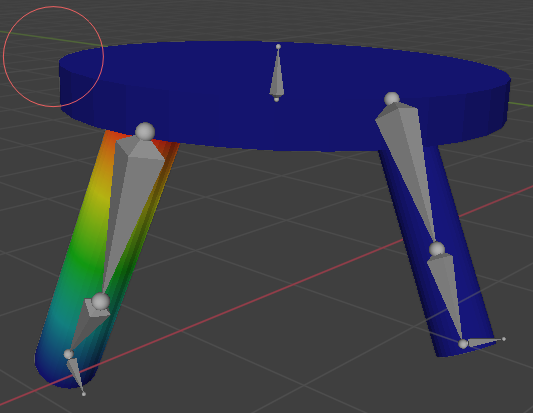
\includegraphics[width=6cm]{figure/pesi.png}
     \caption{Pesi assegnati alla mesh} \label{fig:scheletro}
\end{center}
\end{figure}

\subsection{Collegamento mesh-scheletro e gestione delle deformazioni}
Dopo il trasferimento dei pesi, la mesh viene collegata al rig mediante un modificatore di tipo \textit{Armature}, che permette a Blender di calcolare in tempo reale la deformazione dei vertici in base ai movimenti delle ossa.
Questo collegamento è del tutto automatico e viene completato senza intervento manuale, risultando in un processo di skinning completamente automatizzato.

L'efficacia del metodo è stata verifica attraverso test di animazione, applicando cicli di camminata e movimenti dinamici. I risultati mostrano che la deformazione delle gambe avviene in maniera stabile e coerente, con una buona trasmissione del movimento anche su modelli privi di articolazioni naturali.



\section{Retargeting su oggetti inanimati}

Dopo la fase di rigging e di skinning automatico, in cui è stato generato e collegato lo scheletro al modello tridimensionale del piatto, la fase successiva ha riguardato l'\textbf{applicazione del movimento animato}.
In particolare, l'obiettivo è stato quello di \textbf{trasferire un'animazione umanoide preesistente}, proveniente da una sorgente esterna (come Mixamo), al modello personalizzato realizzato in Blender.

Questa operazione, nota come \textbf{retargeting dell'animazione}, consiste nel mappare i movimenti di un rig sorgente su un rig di destinazione avente una struttura scheletrica diversa, ma compatibile a livello gerarchico.
Nel contesto di questo lavoro, il retargeting ha permesso di riutilizzare animazioni di camminata o corsa tipiche di personaggi umanoidi per animare oggetti non convenzionati, come il \textit{piatto} o la \textit{tazzina con gambe}, generando un effetto dinamico coerente senza dover ricorrere a un'animazione manuale.

Il processo è stato sviluppato interamente in \textbf{Blender}, attraverso \textbf{script Python dedicati}, che automatizzano la fase di assegnazione dei vincoli di trasformazione tra rig sorgente e rig target. Questa automazione ha reso possibile un trasferimento accurato delle animazioni anche in presenza di differenze morfologiche significative tra i modelli, mantenendo la coerenza strutturale e la stabilità del movimento. I passaggi specifici per questo processo di retargeting su oggetti inanimati sono riassunti nell'Algorithm~\ref{alg:cap}.

\vspace{5mm}
\begin{minipage}{1\linewidth}
\begin{algorithm}[H]
\caption{RetargetAnimation} \label{alg:cap}
\KwIn{sourceRig, targetRig}
\tcp{sourceRig: armatura sorgente, targetRig: armatura di destinazione}
\ForEach{bone $t$ in targetRig}{
\tcp{Itera su tutte le ossa del rig di destinazione}
    $s \leftarrow$ sourceRig.getBone(t.name)\;
    \tcp{Ricerca dell'osso omonimo nel rig sorgente}
    \If{$s$ exists}{
        apply CopyLocation($s \rightarrow t$)\;
        \tcp{Copia la posizione dell'osso sorgente sull'osso target}
        
        apply CopyRotation($s \rightarrow t$)\;
        \tcp{Copia la rotazione dell'osso sorgente sull'osso target}
    }
}
\end{algorithm}
\end{minipage}


\subsection{Trasferimento di animazioni umanoidi agli oggetti}

Per permettere al modello non antropomorfo di riprodurre i movimenti di un rig umanoide (nel caso specifico, un'animazione di camminata proveniente da Mixamo), è stato realizzato un sistema di \textbf{retargeting automatico} all'interno di Blender tramite script Python.

L'obiettivo è mappare le ossa del rig sorgente (umanoide) su quelle di rig target (nel nostro caso il \textit{PiattoRig}), trasferendo posizioni e rotazioni delle articolazioni principali. Questo processo è stato implementato utilizzando \textbf{vincoli di trasformazione} (constraints) che permettono di copiare in tempo reale i movimenti del rig originale.

In particolare, per ciascun osso del rig del piatto, lo script aggiunge vincoli principali:

\begin{itemize}
    \item \textbf{Copy Location}, per copiare la posizione locale dell'osso corrispondente;
    \item \textbf{Copy Rotation}, per copiare la rotazione, mantenendo la coerenza con il sistema di coordinate locale.
\end{itemize}


\begin{figure}[H]
\begin{center}
     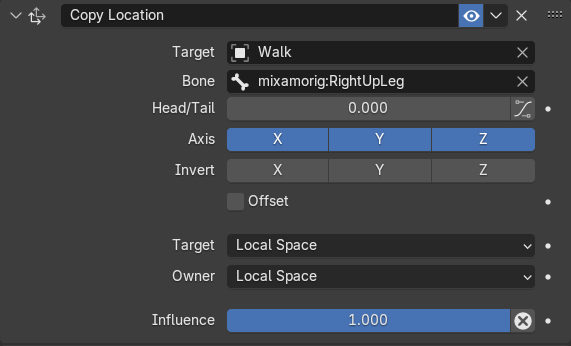
\includegraphics[width=10cm]{figure/copy.png}
     \caption{Vincoli Copy Location su Blender} 
     \label{fig:cop}
\end{center}
\end{figure}

L'approccio consente di sincronizzare i movimenti dell'intero rig, evitando la necessità di keyframe manuali o conversioni di animazioni tra sistemi scheletrici differenti. Un frammento esemplificativo del codice implementato è mostrato di seguito: 
\vspace{5mm} %5mm vertical space

\begin{minted}[fontsize=\small, breaklines]{python}
    for bone in target.pose.bones:
    src_bone = source.pose.bones.get(bone.name)
    if not src_bone:
        continue

    c_loc = bone.constraints.new(type='COPY_LOCATION')
    c_loc.target = source
    c_loc.subtarget = bone.name
    c_loc.owner_space = 'LOCAL'
    c_loc.target_space = 'LOCAL'

    c_rot = bone.constraints.new(type='COPY_ROTATION')
    c_rot.target = source
    c_rot.subtarget = bone.name
    c_rot.owner_space = 'LOCAL'
    c_rot.target_space = 'LOCAL'
\end{minted}
\captionof{listing}{Script per la copia dei vincoli di posizione e rotazione tra armature.}

\vspace{5mm} %5mm vertical space
Questo frammento mostra la parte centrale dello script, in cui ad ogni osso viene assegnata una relazione diretta di copia di posizione e rotazione rispetto all'omologo del rig sorgente. Il risultato è un trasferimento fedele del movimento, applicato anche a oggetti con una morfologia completamente diversa da quella del modello originale.

\subsection{Gestione del movimento coerente (root motion o offset spaziali)}

Per garantire che l'oggetto animato mantenga un movimento coerente nello spazio, è stata introdotta una seconda fase di \textbf{controllo del root motion}, ovvero della traslazione globale del rig.

Il problema principale riscontrato riguarda l'osso radice (\textit{mixamorig:Hips}), che un rig umanoide controlla lo spostamento complessivo del corpo. Nel caso di un oggetto statico come il piatto, la riproduzione diretta di tale movimento avrebbe causato uno spostamento dell'intero modello lungo l'asse verticale.

\vspace{5mm}
\begin{minipage}{1\linewidth}
\begin{algorithm}[H]
\caption{ApplyRootMotionFiltering} \label{alg2:cap}
\KwIn{sourceHips, targetHips}
\tcp{sourceHips: osso dei fianchi dell’armatura sorgente}
\tcp{targetHips: osso dei fianchi dell’armatura di destinazione}
CopyRotation(sourceHips $\rightarrow$ targetHips)\;
\tcp{Copia la rotazione dell’osso delle anche dalla sorgente al target}
CopyLocation(sourceHips $\rightarrow$ targetHips)\;
\tcp{Copia la traslazione dell’osso delle anche dalla sorgente al target}
DisableZAxisTranslation(targetHips)\;
\tcp{Disabilita la traslazione lungo l’asse verticale (Z) sul target, evitando movimenti indesiderati in altezza}

\end{algorithm}
\end{minipage}
\vspace{5mm}

Per risolvere questo problema, è stato utilizzato un secondo script che gestisce selettivamente il trasferimento delle trasformazioni, limitando il movimento all'asse orizontale (X e Y) e impedendo la traslazione lungo l'asse Z. La logica dell'algoritmo è riassunta nell'Algorithm~\ref{alg2:cap}, che ne evidenzia i passaggi principali.
\vspace{2mm} %5mm vertical space
\begin{minted}[fontsize=\small, breaklines]{python}
    hips = target.pose.bones.get("mixamorig:Hips")
    if hips:
        c_loc = hips.constraints.new(type='COPY_LOCATION')
        c_loc.target = source
        c_loc.subtarget = "mixamorig:Hips"
        c_loc.owner_space = 'WORLD'
        c_loc.target_space = 'WORLD'
        c_loc.use_z = False  # non copiare l'altezza (Z)
    
        c_rot = hips.constraints.new(type='COPY_ROTATION')
        c_rot.target = source
        c_rot.subtarget = "mixamorig:Hips"
\end{minted}
\captionof{listing}{Script che cerca di evitare le deformazioni quando viene trasferito il movimento.}
\vspace{5mm} %5mm vertical space
Questa configurazione consente di preservare il \textbf{movimento orizzontale} del rig, mantenendo però fisso il punto di contatto del modello con il suolo. Il risultato è un'animazione fluida e coerente, dove il piatto segue la dinamica della camminata umanoide senza perdere l'allineamento spaziale.

